\chapter{Baterias, células a combustível e eletrólise}\label{ch:b2:batteries-electrolysis}

Cada quilograma de alumínio extraído de seu minério consome cerca de
\qty{13}{kW.h} de eletricidade; fundir um quilograma de sucata exige, em
princípio, os \qty{0.3}{kW.h} que o aquecem até seu ponto de fusão e o
fundem. A diferença é o trabalho de uma longa fileira de cubas de \omterm{def:b2:batteries-electrolysis:electrolysis}{eletrólise},
cada uma fazendo passar centenas de milhares de ampères por um sal fundido
sob alguns volts. Uma bateria funciona no sentido inverso: uma reação
espontânea impulsiona a corrente. Com as \omterm{def:b2:current-potential-curves:ie-curve}{curvas corrente--potencial} do
\cref{ch:b2:current-potential-curves}, ambas se leem no mesmo diagrama, assim
como um pedaço de zinco que se dissolve em ácido.
% ledger: hT:Al_l.933, aw:Al

\begin{recall}
\Cref{ch:b2:cell-thermodynamics}: $\Delta_r G = -nFE$, o trabalho máximo, a
\omterm{def:b2:cell-thermodynamics:faraday}{constante de Faraday}. \Cref{ch:b2:current-potential-curves}: \omterm{def:b2:current-potential-curves:ie-curve}{curvas
corrente--potencial}, \omterm{def:b2:current-potential-curves:fast-slow}{sistemas rápidos} e lentos, \omterm{def:b2:current-potential-curves:overpotential}{sobretensões}, \omterm{def:b2:current-potential-curves:limiting-current}{correntes
limite}, as barreiras da água. \Cref{ch:b2:ellingham}: por que o alumínio não é
obtido com carbono. O volume escolar: a \omterm{def:b2:batteries-electrolysis:electrolysis}{eletrólise}, os \omterm{def:b2:batteries-electrolysis:battery}{acumuladores}.
\end{recall}

\begin{omfigure}
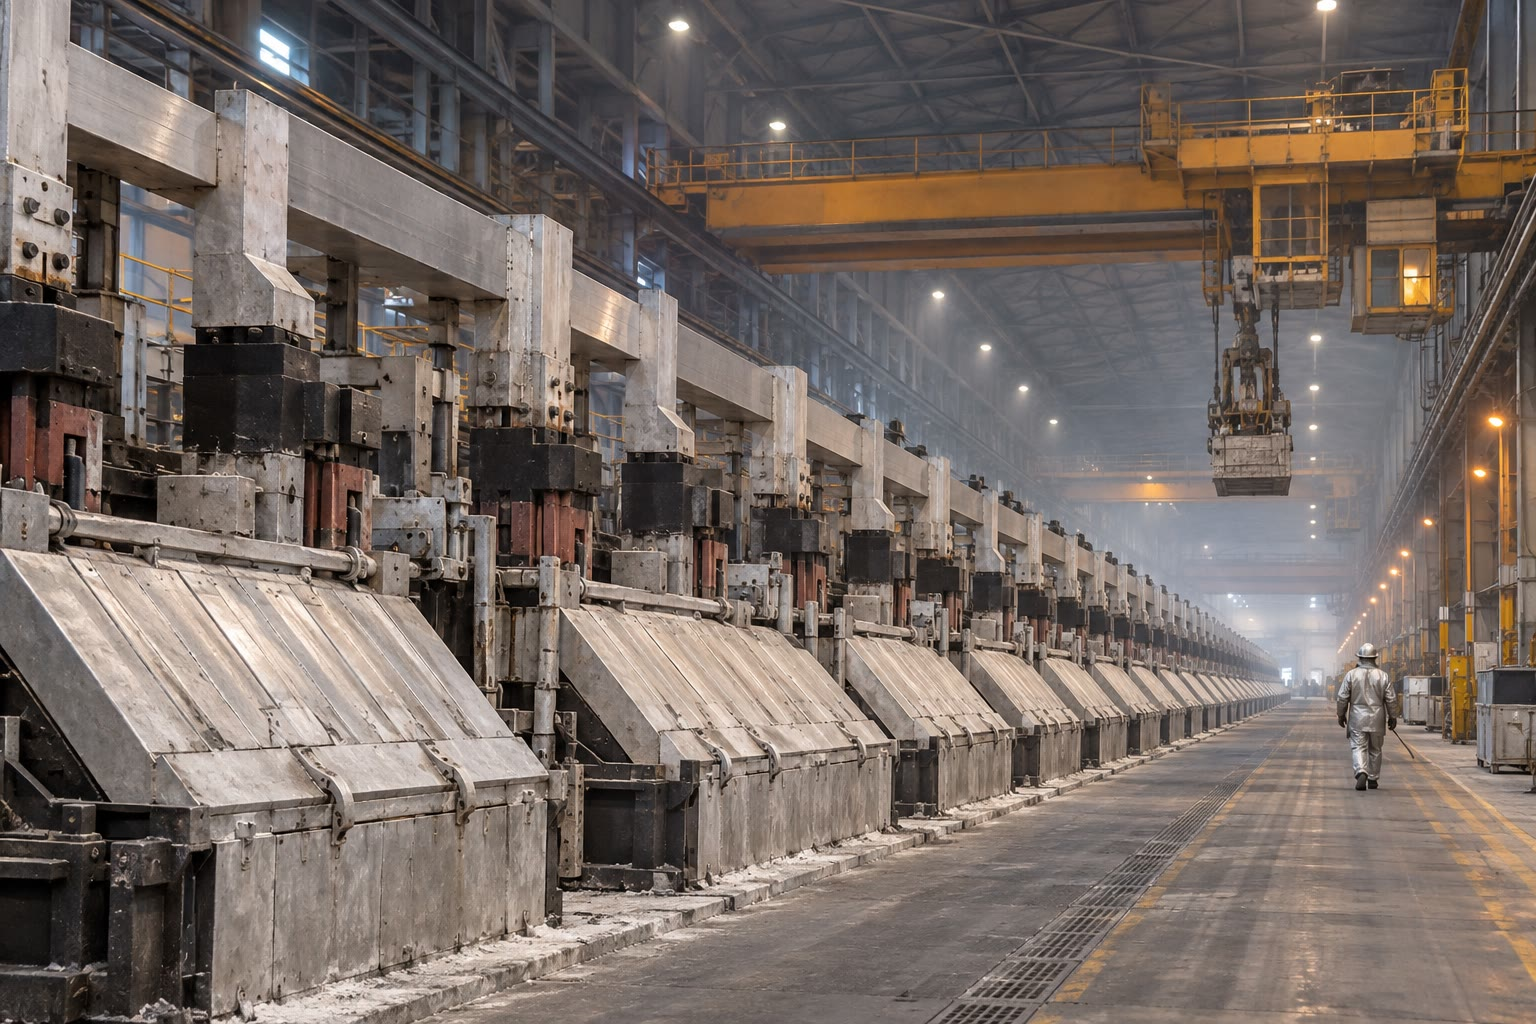
\includegraphics[width=0.62\linewidth]{images/book3/ai/b2-11-potroom.jpg}

{\small A sala de cubas de uma fábrica de alumínio: uma fileira de cubas de
\omterm{def:b2:batteries-electrolysis:electrolysis}{eletrólise}, com centenas de metros de comprimento, ligadas em série; a ponte
rolante troca os ânodos de carbono à medida que eles se consomem.}
\end{omfigure}

\section{Reações espontâneas lidas nas curvas}

\begin{definition}[Potencial misto]\label{def:b2:batteries-electrolysis:mixed-potential}
O \emph{potencial misto}\index{potencial misto} de um eletrodo sobre o qual reagem
dois pares diferentes, um oxidado e outro reduzido, é o potencial que ele
assume quando não circula corrente líquida: a \omterm{def:b2:current-potential-curves:ie-curve}{corrente anódica} de um par é
então igual e oposta à \omterm{def:b2:current-potential-curves:ie-curve}{corrente catódica} do outro.
\end{definition}

\begin{proposition}[Um metal em uma solução]\label{prop:b2:batteries-electrolysis:mixed}
Um metal mergulhado em uma solução capaz de oxidá-lo se estabiliza no
potencial $E_m$ em que $i_a(E_m) = -i_c(E_m)$, a \omterm{def:b2:current-potential-curves:ie-curve}{corrente anódica} da oxidação
do metal equilibrando a \omterm{def:b2:current-potential-curves:ie-curve}{corrente catódica} da redução do oxidante; o metal se
dissolve com a velocidade $i_a(E_m)/(nF)$.
\end{proposition}

\begin{proof}
Um pedaço de metal isolado não transporta corrente líquida. As duas
semirreações ocorrem em sua superfície ao mesmo potencial; logo suas correntes,
lidas em suas curvas nesse potencial, somam zero. Pela
\cref{prop:b2:current-potential-curves:current-rate}, a \omterm{def:b2:current-potential-curves:ie-curve}{corrente anódica} dá a
velocidade de oxidação.
\end{proof}

\begin{omfigure}
\begin{tikzpicture}
\begin{axis}[omie, width=0.82\linewidth, height=6cm, xmin=-1.1, xmax=-0.3,
  ymin=-3, ymax=3, xlabel={$E$ (V)}, ylabel={$i$}, clip=true, clip mode=individual,
  axis y line=left]
\addplot[omanodic] table[x=E, y=i] {figdata/out/bachelor-2-ie-curves-f-Zn.dat};
\addplot[omcathodic] table[x=E, y=i] {figdata/out/bachelor-2-ie-curves-f-HZn.dat};
\addplot[omcathodic, dashed] table[x=E, y=i] {figdata/out/bachelor-2-ie-curves-f-HCu.dat};
\draw[densely dotted] (axis cs:-0.820,-0.148) -- (axis cs:-0.820,0.148);
\draw[densely dotted] (axis cs:-0.737,-2.38) -- (axis cs:-0.737,2.38);
\fill (axis cs:-0.820,0.148) circle (1.3pt); \fill (axis cs:-0.737,2.38) circle (1.3pt);
\node[font=\scriptsize, anchor=south east] at (axis cs:-0.825,0.2) {zinco sozinho};
\node[font=\scriptsize, anchor=west] at (axis cs:-0.73,2.38) {zinco em contato com cobre};
\node[font=\scriptsize, omThm, anchor=west] at (axis cs:-0.70,1.2) {\ce{Zn} $\to$ \ce{Zn^2+}};
\node[font=\scriptsize, omDef, anchor=north west, align=left] at (axis cs:-0.87,-0.5) {\ce{H+} $\to$ \ce{H2}\\ sobre zinco};
\node[font=\scriptsize, omDef, anchor=north west] at (axis cs:-0.66,-1.7) {sobre cobre};
\end{axis}
\end{tikzpicture}

{\small Zinco em ácido (curvas modelo, íons zinco diluídos; potenciais de
$-1.1$ a \qty{-0.3}{V}). Sozinho, o zinco se estabiliza no
\omterm{def:b2:batteries-electrolysis:mixed-potential}{potencial misto} em que sua oxidação equilibra a redução lenta de \ce{H+}
sobre o zinco: uma corrente pequena, uma dissolução lenta. Em contato com o
cobre, sobre o qual a redução de \ce{H+} é menos lenta, o equilíbrio passa a
um potencial mais alto e a uma corrente mais de dez vezes maior: o zinco se
dissolve depressa, e o hidrogênio borbulha sobre o cobre.}
\end{omfigure}

A mesma leitura explica a corrosão (\cref{ch:b2:corrosion}): a velocidade de
corrosão de um metal é a corrente em seu \omterm{def:b2:batteries-electrolysis:mixed-potential}{potencial misto}.

\section{Pilhas que fornecem corrente}

\begin{definition}[Baterias]\label{def:b2:batteries-electrolysis:battery}
Uma \emph{pilha primária}\index{pilha primaria@pilha primária} é uma pilha eletroquímica usada
uma única vez, até que seus reagentes se esgotem. Um \emph{acumulador}\index{acumulador}
é uma pilha que pode ser recarregada forçando-se uma corrente através dela no
sentido inverso, o que inverte sua reação. A \emph{energia
específica}\index{energia especifica@energia específica} de uma pilha é a energia elétrica que
ela fornece por unidade de massa, em geral em \unit{W.h/kg}.
\end{definition}

\begin{proposition}[Tensão de uma pilha que fornece corrente]\label{prop:b2:batteries-electrolysis:delivering}
Uma pilha que fornece uma corrente $I$ tem uma tensão
\[
  U = E_+ - E_- - \eta_a - |\eta_c| - rI ,
\]
em que $E_+$ e $E_-$ são os potenciais de equilíbrio de seus dois eletrodos,
$\eta_a > 0$ a \omterm{def:b2:current-potential-curves:overpotential}{sobretensão} da oxidação no eletrodo negativo,
$\eta_c < 0$ a da redução no eletrodo positivo, e $r$ a
resistência interna (eletrólito, separador, conexões).
\end{proposition}

\begin{proof}
A mesma corrente $I$ é anódica no eletrodo negativo, cujo potencial é lido
em sua curva anódica, $E_- + \eta_a$, e catódica no positivo, cujo potencial
é $E_+ + \eta_c$. Entre eles, a corrente atravessa o eletrólito, onde o
potencial cai de $rI$. Logo $U = (E_+ + \eta_c) - (E_- +
\eta_a) - rI$.
\end{proof}

\begin{omfigure}
\begin{tikzpicture}
\begin{axis}[omie, width=0.82\linewidth, height=5.6cm, xmin=-1.2, xmax=0.8,
  ymin=-2, ymax=2, xlabel={$E$ (V)}, ylabel={$i$}, clip=true, clip mode=individual]
\addplot[omanodic] table[x=E, y=i] {figdata/out/bachelor-2-ie-curves-h-neg.dat};
\addplot[omcathodic] table[x=E, y=i] {figdata/out/bachelor-2-ie-curves-h-pos.dat};
\draw[densely dashed, gray] (axis cs:-1.2,1) -- (axis cs:0.8,1);
\draw[densely dashed, gray] (axis cs:-1.2,-1) -- (axis cs:0.8,-1);
\node[font=\scriptsize, gray, anchor=south west] at (axis cs:-1.18,1) {$+I$};
\node[font=\scriptsize, gray, anchor=north west] at (axis cs:-1.18,-1) {$-I$};
\fill (axis cs:-0.730,1) circle (1.3pt); \fill (axis cs:0.210,-1) circle (1.3pt);
\draw[densely dotted] (axis cs:-0.85,0) -- (axis cs:-0.85,0.5);
\draw[densely dotted] (axis cs:0.45,0) -- (axis cs:0.45,-0.5);
\node[font=\scriptsize, anchor=south] at (axis cs:-0.85,0.5) {$E_-$};
\node[font=\scriptsize, anchor=north] at (axis cs:0.45,-0.5) {$E_+$};
\draw[<->, thick, omProp] (axis cs:-0.730,1.5) -- (axis cs:0.210,1.5) node[midway, above, font=\scriptsize] {$U + rI$};
\draw[densely dotted] (axis cs:-0.730,1) -- (axis cs:-0.730,1.5);
\draw[densely dotted] (axis cs:0.210,-1) -- (axis cs:0.210,1.5);
\node[font=\scriptsize, omThm, anchor=west] at (axis cs:-0.70,0.6) {eletrodo negativo};
\node[font=\scriptsize, omDef, anchor=west] at (axis cs:0.30,-1.5) {eletrodo positivo};
\end{axis}
\end{tikzpicture}

{\small O ponto de funcionamento de uma pilha (curvas modelo). A uma corrente
$I$, o eletrodo negativo fica em sua curva anódica e o positivo em sua curva
catódica; a diferença entre os dois potenciais, menos a queda ôhmica $rI$, é
a tensão fornecida. Ela cai à medida que $I$ aumenta.}
\end{omfigure}

\begin{method}[O ponto de funcionamento de uma pilha ou de um eletrolisador]\label{met:b2:batteries-electrolysis:operating-point}
\begin{enumerate}
  \item Trace a curva anódica do eletrodo que é oxidado e a curva catódica do
        que é reduzido.
  \item Para uma corrente $I$, leia o potencial de cada eletrodo em $+I$ na
        curva anódica e em $-I$ na curva catódica.
  \item A diferença entre os dois potenciais, corrigida de $rI$ (subtraído
        para uma pilha, somado para um \omterm{def:b2:batteries-electrolysis:electrolysis}{eletrolisador}), é a tensão.
\end{enumerate}
\end{method}

\begin{example}[O acumulador de chumbo-ácido]\label{ex:b2:batteries-electrolysis:lead}
No eletrodo negativo, \ce{Pb + SO4^2- -> PbSO4 + 2e-}; no positivo,
\ce{PbO2 + 4H+ + SO4^2- + 2e- -> PbSO4 + 2H2O}. No total,
\[
  \ce{Pb + PbO2 + 4H+ + 2SO4^2- -> 2PbSO4 + 2H2O},
\]
$\Delta_r G^\circ = 2(-813.14) + 2(-237.13) - (-217.33) - 2(-744.53) =
\qty{-394.1}{kJ/mol}$, $E^\circ = 394\,100/(2 \times 96\,485) = \qty{2.04}{V}$.
Os dois eletrodos se recobrem de sulfato de chumbo durante a descarga; a carga
inverte a reação. A redução de \ce{H+} sobre o chumbo e a oxidação da água
sobre o dióxido de chumbo são lentas: é por isso que uma pilha de \qty{2}{V}
pode ser carregada na água, cuja janela termodinâmica tem apenas
\qty{1.23}{V} de largura.
% ledger: dfg:PbSO4_cr, dfg:H2O_l, dfg:PbO2_cr, dfg:SO42-_ao
\end{example}

\begin{omfigure}
\begin{tikzpicture}[font=\small, >={Stealth}]
  \draw[thick] (0,0) rectangle (6,3.2);
  \fill[omDef!10] (0.05,0.05) rectangle (5.95,2.7);
  \fill[black!45] (0.6,0.4) rectangle (1.1,2.9);
  \fill[brown!60!black] (4.9,0.4) rectangle (5.4,2.9);
  \draw[thick] (0.85,2.9) -- (0.85,3.9) node[pos=0.75, left] {$-$};
  \draw[thick] (5.15,2.9) -- (5.15,3.9) node[pos=0.75, right] {$+$};
  \draw[->, thick, omProp] (0.85,3.9) -- (0.85,4.3) -- (5.15,4.3) -- (5.15,3.95);
  \node[font=\scriptsize, omProp, anchor=south] at (3,4.3) {$\mathrm{e^-}$ na descarga};
  \node[font=\scriptsize, align=center] at (0.85,-0.45) {\ce{Pb}\\ (\ce{PbSO4} na descarga)};
  \node[font=\scriptsize, align=center] at (5.15,-0.45) {\ce{PbO2}\\ (\ce{PbSO4} na descarga)};
  \node[font=\scriptsize, align=center] at (3.0,1.6) {solução de \ce{H2SO4}\\ \ce{H+}, \ce{HSO4-}, \ce{SO4^2-}};
\end{tikzpicture}

{\small O \omterm{def:b2:batteries-electrolysis:battery}{acumulador} de chumbo-ácido, esquemático. Na descarga, o chumbo é
oxidado e o dióxido de chumbo reduzido, ambos a sulfato de chumbo, e o ácido é
consumido: a massa específica da solução indica o estado de carga.}
\end{omfigure}

\begin{omfigure}
\begin{tikzpicture}[font=\small, >={Stealth}]
  \draw[thick] (0,0) rectangle (7,3);
  % graphite layers
  \foreach \y in {0.5,0.9,1.3,1.7,2.1,2.5} \draw[thick, black!70] (0.3,\y) -- (2.3,\y);
  \foreach \y in {0.7,1.1,1.5,1.9,2.3} \foreach \x in {0.6,1.3,2.0} \fill[omDef] (\x,\y) circle (0.07);
  % layered oxide
  \foreach \y in {0.5,0.9,1.3,1.7,2.1,2.5} \draw[thick, omThm] (4.7,\y) -- (6.7,\y);
  \foreach \y in {0.7,1.5,2.3} \foreach \x in {5.0,5.7,6.4} \fill[omDef] (\x,\y) circle (0.07);
  \draw[densely dashed] (3.5,0) -- (3.5,3);
  \node[font=\scriptsize, align=center] at (1.3,-0.45) {grafita (negativo)};
  \node[font=\scriptsize, align=center] at (5.7,-0.45) {óxido lamelar (positivo)};
  \node[font=\scriptsize, anchor=south] at (3.5,3.0) {separador};
  \draw[->, thick, omThm] (2.5,2.1) -- (4.5,2.1) node[midway, above, font=\scriptsize, fill=white, inner sep=1pt] {\ce{Li+} na descarga};
  \draw[<-, thick, omDef] (2.5,0.9) -- (4.5,0.9) node[midway, below, font=\scriptsize, fill=white, inner sep=1pt] {\ce{Li+} na carga};
\end{tikzpicture}

{\small Uma célula de íon-lítio, esquemática. Os íons lítio (pontos azuis)
ficam entre as camadas da grafita na célula carregada; na descarga, eles
atravessam o eletrólito para se intercalar entre as camadas de um óxido
metálico, enquanto os elétrons percorrem o circuito externo. Nenhum eletrodo
se dissolve ou se deposita: os íons vão e vêm entre dois hospedeiros.}
\end{omfigure}

\begin{history}[A pilha de Volta]
\begin{minipage}[t]{0.27\linewidth}
\vspace{0pt}
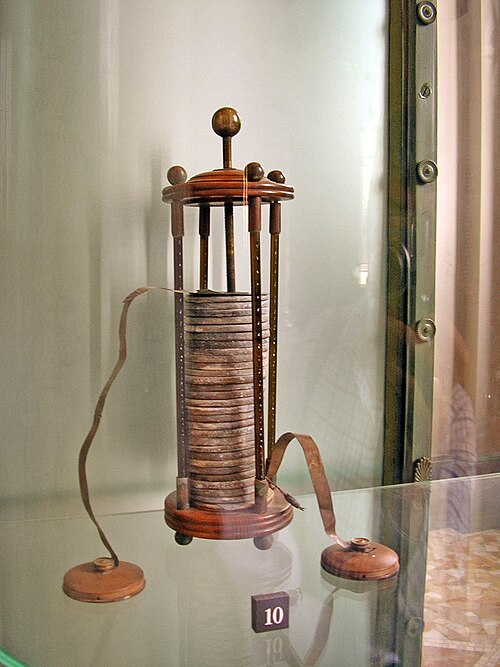
\includegraphics[width=\linewidth]{images/book3/volta-pile.jpg}
\end{minipage}\hfill
\begin{minipage}[t]{0.69\linewidth}
\vspace{0pt}
Em 1800, Alessandro Volta descreveu uma coluna de discos de dois metais
diferentes, zinco e cobre ou prata, separados por pano embebido em salmoura:
a primeira fonte de uma corrente elétrica contínua. Em poucas semanas, outros
a usaram para decompor a água e, em uma década, Humphry Davy havia isolado o
sódio e o potássio por \omterm{def:b2:batteries-electrolysis:electrolysis}{eletrólise} de seus hidróxidos fundidos com uma grande
pilha. A fotografia mostra uma das pilhas do próprio Volta. (Fotografia:
GuidoB, CC BY-SA 3.0, Wikimedia Commons.)
\end{minipage}
\end{history}

\section{Células a combustível}

\begin{definition}[Célula a combustível]\label{def:b2:batteries-electrolysis:fuel-cell}
Uma \emph{célula a combustível}\index{celula a combustivel@célula a combustível} é uma pilha cujos
reagentes, um combustível e um oxidante (em geral o oxigênio do ar), são
alimentados continuamente a seus eletrodos e cujos produtos são retirados, de
modo que ela fornece corrente enquanto for alimentada.
\end{definition}

Na célula com membrana de troca de prótons do ônibus do
\cref{ch:b2:cell-thermodynamics}, o hidrogênio é oxidado sobre um catalisador
de platina, \ce{H2 -> 2H+ + 2e-}, os prótons atravessam uma fina membrana de
polímero ácido, e o oxigênio é reduzido do outro lado, \ce{O2 + 4H+ + 4e- -> 2H2O}.
A oxidação do hidrogênio sobre a platina é um \omterm{def:b2:current-potential-curves:fast-slow}{sistema rápido}; a redução do
oxigênio é lenta sobre qualquer eletrodo. A maior parte da tensão perdida
entre os \qty{1.23}{V} da célula reversível e a tensão de trabalho é a
\omterm{def:b2:current-potential-curves:overpotential}{sobretensão} do eletrodo de oxigênio; o resto, a resistência da membrana e, em
corrente alta, o suprimento de oxigênio ao catalisador (uma \omterm{def:b2:current-potential-curves:limiting-current}{corrente limite}).

\section{Eletrólise}

\begin{definition}[Eletrólise]\label{def:b2:batteries-electrolysis:electrolysis}
Uma \emph{eletrólise}\index{eletrolise@eletrólise} é uma reação redox não espontânea
forçada por uma corrente fornecida por um gerador externo; a cuba em que ela
ocorre é um \emph{eletrolisador}\index{eletrolisador}. O ânodo, onde ocorre a
oxidação, é ligado ao polo positivo do gerador.
\end{definition}

\begin{proposition}[Tensão mínima termodinâmica]\label{prop:b2:batteries-electrolysis:minimum-voltage}
Uma \omterm{def:b2:batteries-electrolysis:electrolysis}{eletrólise} cuja reação tem $\Delta_r G > 0$ exige uma tensão de no
mínimo $\Delta_r G/(nF)$.
\end{proposition}

\begin{proof}
O gerador fornece o trabalho $nFU$ por mol de reação; pelo
\cref{thm:b2:cell-thermodynamics:delta-g-nfe} aplicado à reação inversa, o
trabalho elétrico recebido deve ser no mínimo $\Delta_r G$.
\end{proof}

\begin{proposition}[Tensão de um eletrolisador]\label{prop:b2:batteries-electrolysis:electrolysis-voltage}
Um \omterm{def:b2:batteries-electrolysis:electrolysis}{eletrolisador} percorrido por uma corrente $I$ exige
\[
  U = (E_a - E_c) + \eta_a + |\eta_c| + rI ,
\]
sendo $E_a$, $E_c$ os potenciais de equilíbrio dos pares do ânodo e do cátodo
($E_a - E_c = \Delta_r G/(nF)$), $\eta_a$, $\eta_c$ suas \omterm{def:b2:current-potential-curves:overpotential}{sobretensões} a essa
corrente e $r$ a resistência entre os eletrodos.
\end{proposition}

\begin{proof}
Como para uma pilha, a mesma corrente é anódica no ânodo, ao potencial $E_a +
\eta_a$, e catódica no cátodo, a $E_c + \eta_c$; o gerador também precisa
fazê-la atravessar o eletrólito, o que acrescenta $rI$.
\end{proof}

\begin{method}[Prever uma eletrólise]\label{met:b2:batteries-electrolysis:predict-electrolysis}
\begin{enumerate}
  \item Liste todas as espécies que podem ser oxidadas no ânodo (incluindo o
        metal do ânodo e o solvente) e todas as que podem ser reduzidas no
        cátodo (incluindo o solvente).
  \item Trace suas \omterm{def:b2:current-potential-curves:ie-curve}{curvas corrente--potencial} sobre os materiais de eletrodo usados.
  \item À medida que a tensão aumenta, a primeira curva anódica e a primeira
        curva catódica atingidas dão as reações; em correntes maiores, as
        seguintes acrescentam as suas.
\end{enumerate}
\end{method}

\begin{definition}[Rendimento faradaico]\label{def:b2:batteries-electrolysis:faradaic-efficiency}
O \emph{rendimento faradaico}\index{rendimento faradaico} $\eta_F$ de uma
\omterm{def:b2:batteries-electrolysis:electrolysis}{eletrólise} é a fração da carga que passou que forma o produto desejado. Seu
\emph{consumo específico de energia}\index{consumo especifico de energia@consumo específico de energia}
é a energia elétrica usada por unidade de massa de produto.
\end{definition}

\begin{proposition}[Lei de Faraday]\label{prop:b2:batteries-electrolysis:faraday-mass}
Uma corrente $I$ que passa durante um tempo $t$ com \omterm{def:b2:batteries-electrolysis:faradaic-efficiency}{rendimento faradaico}
$\eta_F$ produz uma massa $m = \eta_F MIt/(nF)$ de um produto de massa molar
$M$ formado com $n$ elétrons por mol.
\end{proposition}

\begin{proof}
A carga $It$, da qual $\eta_F It$ forma o produto, corresponde, pela
\cref{prop:b2:cell-thermodynamics:charge}, a $\eta_F It/(nF)$ mols.
\end{proof}

\begin{proposition}[Energia por quilograma]\label{prop:b2:batteries-electrolysis:energy}
Sob uma tensão $U$ e com \omterm{def:b2:batteries-electrolysis:faradaic-efficiency}{rendimento faradaico} $\eta_F$, o \omterm{def:b2:batteries-electrolysis:faradaic-efficiency}{consumo específico
de energia} é $w = nFU/(\eta_F M)$.
\end{proposition}

\begin{proof}
A energia é $UIt$ e a massa, $\eta_F MIt/(nF)$; divida.
\end{proof}

\section{Eletrólises industriais}

\paragraph{Zinco.} A maior parte do zinco é obtida por \omterm{def:b2:batteries-electrolysis:electrolysis}{eletrólise} da solução
ácida de sulfato de zinco do \cref{ch:b2:ellingham}. O zinco se deposita no
cátodo embora \ce{H+} seja o oxidante mais forte: sobre o zinco, a redução de
\ce{H+} é muito lenta, e a onda do zinco é atingida primeiro; o ânodo libera
oxigênio.

\begin{omfigure}
\begin{tikzpicture}
\begin{axis}[omie, width=0.82\linewidth, height=5.6cm, xmin=-1.6, xmax=2.4,
  ymin=-2.4, ymax=2.4, xlabel={$E$ (V)}, ylabel={$i$}, clip=true, clip mode=individual]
\addplot[omcathodic] table[x=E, y=i] {figdata/out/bachelor-2-ie-curves-g-cath.dat};
\addplot[omanodic] table[x=E, y=i] {figdata/out/bachelor-2-ie-curves-g-an.dat};
\draw[densely dotted] (axis cs:-0.76,-2.2) -- (axis cs:-0.76,0.4);
\draw[densely dotted] (axis cs:0,-2.2) -- (axis cs:0,0.4);
\node[font=\scriptsize, anchor=south] at (axis cs:-0.76,0.4) {$-0.76$};
\node[font=\scriptsize, anchor=south east] at (axis cs:-0.02,0.4) {$0$};
\node[font=\scriptsize, omDef, anchor=north west, align=left] at (axis cs:-0.7,-1.05) {\ce{Zn^2+} $\to$ \ce{Zn},\\ patamar};
\node[font=\scriptsize, omDef, anchor=east, align=right] at (axis cs:-1.32,-0.9) {\ce{H+} $\to$ \ce{H2}\\ sobre Zn};
\node[font=\scriptsize, omThm, anchor=east] at (axis cs:1.85,1.6) {\ce{H2O} $\to$ \ce{O2}};
\node[font=\scriptsize, gray, align=center] at (axis cs:-0.38,-0.5) {aqui, sem \ce{H2}\\ sobre o Zn};
\end{axis}
\end{tikzpicture}

{\small \omterm{def:b2:batteries-electrolysis:electrolysis}{Eletrólise} de uma solução ácida de sulfato de zinco com cátodo de
zinco (curvas modelo). Embora o par \ce{H+}/\ce{H2} ($\qty{0}{V}$) fique acima
de \ce{Zn^2+}/\ce{Zn} ($\qty{-0.76}{V}$), a redução de \ce{H+} sobre o zinco
não começa antes de cerca de \qty{-1.1}{V}: entre os dois, só o zinco se
deposita. No ânodo, a água é oxidada a oxigênio.}
\end{omfigure}

\paragraph{Cloro e hidróxido de sódio.} A salmoura é eletrolisada em uma cuba
dividida por uma membrana que só deixa passar cátions. No ânodo, o cloreto é
oxidado, \ce{2Cl- -> Cl2 + 2e-}; no cátodo, a água é reduzida, \ce{2H2O +
2e- -> H2 + 2OH-}; os íons sódio atravessam a membrana para equilibrar a carga,
e uma solução de hidróxido de sódio sai do lado do cátodo, isenta de cloreto.
O mínimo termodinâmico é $\Delta_r G/(2F) = \qty{2.19}{V}$ para \ce{2Cl- + 2H2O -> Cl2 +
H2 + 2OH-} em condições padrão. O cloro se forma no ânodo no lugar do
oxigênio, embora o par \ce{O2}/\ce{H2O} fique mais abaixo: a oxidação da água
é a mais lenta das duas sobre os materiais de ânodo utilizados.
% ledger: dfg:OH-_ao, dfg:Cl-_ao, dfg:H2O_l

\begin{omfigure}
\begin{tikzpicture}[font=\small, >={Stealth}]
  \draw[thick] (0,0) rectangle (6,3.4);
  \draw[thick, dashed, omProp] (3,0) -- (3,3.4);
  \fill[black!30] (0.4,0.3) rectangle (0.7,3.0);
  \fill[black!50] (5.3,0.3) rectangle (5.6,3.0);
  \node[font=\scriptsize] at (0.55,3.3) {$+$};
  \node[font=\scriptsize] at (5.45,3.3) {$-$};
  \node[font=\scriptsize, align=center] at (1.85,1.9) {salmoura\\ \ce{2Cl-} $\to$\\ \ce{Cl2 + 2e-}};
  \node[font=\scriptsize, align=center] at (4.2,1.9) {solução\\ de \ce{NaOH}\\ \ce{2H2O + 2e-} $\to$\\ \ce{H2 + 2OH-}};
  \draw[->, thick, omDef] (2.6,0.8) -- (3.4,0.8) node[pos=0.1, above, font=\scriptsize] {\ce{Na+}};
  \draw[->, thick] (1.0,3.4) -- (1.0,4.0) node[above] {\ce{Cl2}};
  \draw[->, thick] (5.0,3.4) -- (5.0,4.0) node[above] {\ce{H2}};
  \draw[->, thick] (-0.8,0.6) -- (0,0.6) node[pos=0, left] {entrada de salmoura};
  \draw[->, thick] (6,0.6) -- (6.8,0.6) node[right] {saída de \ce{NaOH}};
  \node[font=\scriptsize, omProp, anchor=north] at (3,-0.05) {membrana de troca de cátions};
\end{tikzpicture}

{\small Uma cuba cloro-álcali a membrana, esquemática. Só os íons sódio
atravessam a membrana; assim o hidróxido formado no cátodo não encontra o cloro.}
\end{omfigure}

\paragraph{Alumínio.} O óxido de alumínio é dissolvido na criolita fundida,
\ce{Na3AlF6}, que funde muito abaixo da alumina, e eletrolisado entre um
cátodo de carbono, sobre o qual se acumula o alumínio líquido, e ânodos de
carbono que se consomem como dióxido de carbono (processo Hall--Héroult):
\[
  \ce{2Al2O3 + 3C -> 4Al + 3CO2} .
\]
O mínimo termodinâmico perto de \qty{1250}{K} é de cerca de \qty{1.18}{V}
(\cref{pb:b2:batteries-electrolysis:1}); a cuba desse problema funciona a três
vezes e meia esse valor, e o excesso se transforma no calor que mantém o
banho fundido.

\begin{omfigure}
\begin{tikzpicture}[font=\small, >={Stealth}]
  \draw[thick, fill=black!12] (0,0) rectangle (7,3.2);
  \fill[black!45] (0.3,0.3) rectangle (6.7,0.8);
  \fill[gray!35] (0.3,0.8) rectangle (6.7,1.4);
  \fill[orange!30] (0.3,1.4) rectangle (6.7,2.5);
  \foreach \x in {1.0,3.0,5.0} {
    \fill[black!75] (\x,1.75) rectangle (\x+1.0,3.6);
    \draw[thick] (\x+0.5,3.6) -- (\x+0.5,4.2);
  }
  \draw[thick] (1.5,4.2) -- (5.5,4.2) node[right] {$+$};
  \node[font=\scriptsize, align=left, anchor=west] at (7.3,2.6) {ânodos de carbono, queimados a \ce{CO2}};
  \node[font=\scriptsize, align=left, anchor=west] at (7.3,1.95) {criolita fundida + \ce{Al2O3} dissolvida};
  \node[font=\scriptsize, align=left, anchor=west] at (7.3,1.1) {alumínio líquido (cátodo)};
  \node[font=\scriptsize, align=left, anchor=west] at (7.3,0.55) {bloco catódico de carbono, $-$};
  \draw[densely dotted] (6.7,2.6) -- (7.3,2.6) (6.7,1.95) -- (7.3,1.95) (6.7,1.1) -- (7.3,1.1) (6.7,0.55) -- (7.3,0.55);
\end{tikzpicture}

{\small Uma cuba Hall--Héroult, corte transversal, esquemático. O alumínio é
reduzido na superfície da poça de metal líquido, que funciona como cátodo; os
íons óxido se descarregam sobre os ânodos de carbono, que eles queimam a
dióxido de carbono.}
\end{omfigure}

\begin{history}[Hall e Héroult, 1886]
\begin{minipage}[t]{0.18\linewidth}
\vspace{0pt}
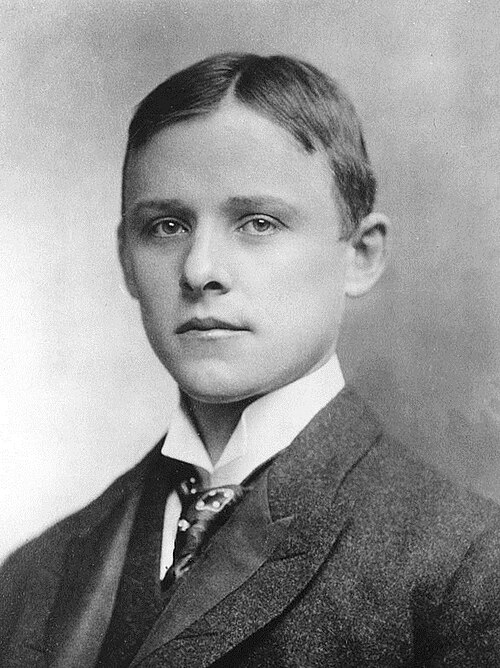
\includegraphics[width=\linewidth]{images/book3/hall.jpg}
\end{minipage}\hspace{0.02\linewidth}%
\begin{minipage}[t]{0.18\linewidth}
\vspace{0pt}
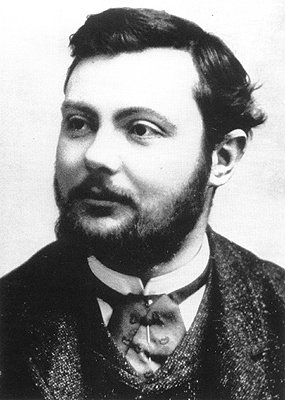
\includegraphics[width=\linewidth]{images/book3/heroult.jpg}
\end{minipage}\hfill
\begin{minipage}[t]{0.58\linewidth}
\vspace{0pt}
Em 1886, aos vinte e dois ou vinte e três anos, Charles Martin Hall e Paul
Héroult, dos dois lados do Atlântico, descobriram independentemente que a
alumina se dissolve na criolita fundida e pode ser eletrolisada ali. O
alumínio, até então um metal precioso obtido reduzindo seu cloreto com
sódio, tornou-se o mais barato dos metais leves assim que a eletricidade
pôde ser gerada em larga escala. (Retratos: Hall, por volta da década de
1880, autor desconhecido, domínio público; Héroult, domínio público;
Wikimedia Commons.)
\end{minipage}
\end{history}

\paragraph{Sódio.} O sódio não pode ser depositado a partir da água, que ele
reduz. Ele é produzido por \omterm{def:b2:batteries-electrolysis:electrolysis}{eletrólise} do cloreto de sódio fundido, cujo ponto
de fusão é abaixado por um sal adicionado (uma \omterm{def:b2:solid-liquid-diagrams:eutectic}{mistura eutética},
\cref{ch:b2:solid-liquid-diagrams}), com o cloro como subproduto. A
\qty{1100}{K}, $\Delta_f G^\circ(\ce{NaCl}, \text{l}) =
\qty{-310.7}{kJ/mol}$: a tensão mínima é de \qty{3.22}{V}.
% ledger: janafG:NaCl.1100

\section{Exercícios}

\begin{exercise}[$\star$]\label{exo:b2:batteries-electrolysis:1}
Na figura do zinco em ácido, leia o \omterm{def:b2:batteries-electrolysis:mixed-potential}{potencial misto} e a corrente do zinco
sozinho e do zinco em contato com o cobre (unidades do modelo), e diga qual
se dissolve mais depressa.
\end{exercise}

\begin{exercise}[$\star$]\label{exo:b2:batteries-electrolysis:2}
Que massa de zinco é depositada em uma hora por uma corrente de \qty{500}{A}
com um \omterm{def:b2:batteries-electrolysis:faradaic-efficiency}{rendimento faradaico} de 100~\%?
\end{exercise}

\begin{exercise}[$\star$]\label{exo:b2:batteries-electrolysis:3}
Calcule a tensão padrão do \omterm{def:b2:batteries-electrolysis:battery}{acumulador} de chumbo-ácido a partir das \omterm{def:b2:reaction-free-energy:gibbs-energy}{energias
de Gibbs} de formação dadas no capítulo, e o número de células de uma bateria
de carro de \qty{12}{V}.
\end{exercise}

\begin{exercise}[$\star$]\label{exo:b2:batteries-electrolysis:4}
Que carga, em ampères-hora, um grama de lítio pode fornecer se for todo
oxidado a \ce{Li+}?
\end{exercise}

\begin{exercise}[$\star\star$]\label{exo:b2:batteries-electrolysis:5}
Uma cuba de refino de cobre faz passar \qty{200}{A} durante \qty{24}{h} e
deposita \qty{5.50}{kg} de cobre. Calcule o \omterm{def:b2:batteries-electrolysis:faradaic-efficiency}{rendimento faradaico}.
\end{exercise}

\begin{exercise}[$\star\star$]\label{exo:b2:batteries-electrolysis:6}
Uma cuba de eletro-obtenção de zinco funciona a \qty{3.3}{V} com um \omterm{def:b2:batteries-electrolysis:faradaic-efficiency}{rendimento
faradaico} de 90~\% (dados do exercício). Calcule a energia elétrica por
quilograma de zinco.
\end{exercise}

\begin{exercise}[$\star\star$]\label{exo:b2:batteries-electrolysis:7}
Uma pilha dá \qty{1.55}{V} a \qty{0.10}{A} e \qty{1.40}{V} a \qty{0.60}{A}.
Supondo desprezíveis as \omterm{def:b2:current-potential-curves:overpotential}{sobretensões}, encontre sua resistência interna e sua
tensão sem corrente.
\end{exercise}

\begin{exercise}[$\star\star$]\label{exo:b2:batteries-electrolysis:8}
A salmoura é eletrolisada na cuba a membrana. Escreva as reações nos
eletrodos, calcule a tensão mínima e explique por que os produtos devem ser
mantidos separados.
\end{exercise}

\begin{exercise}[$\star\star$]\label{exo:b2:batteries-electrolysis:9}
Calcule a tensão mínima para a \omterm{def:b2:batteries-electrolysis:electrolysis}{eletrólise} do cloreto de sódio fundido a
\qty{1100}{K} e a energia mínima por quilograma de sódio.
\end{exercise}

\begin{exercise}[$\star\star\star$]\label{exo:b2:batteries-electrolysis:10}
Usando \omterm{def:b2:current-potential-curves:ie-curve}{curvas corrente--potencial}, explique por que o zinco pode ser
depositado a partir de um banho ácido sobre um cátodo de zinco, e preveja o
que aconteceria sobre um cátodo de platina no início da deposição.
\end{exercise}

\begin{exercise}[$\star\star\star$]\label{exo:b2:batteries-electrolysis:11}
A partir dos $\Delta_f G^\circ$ a \qty{1100}{K} e \qty{1300}{K} ($\ce{Al2O3}$: $-1328.3$ e
$-1262.3$; $\ce{CO2}$: $-396.0$ e $-396.2$ \unit{kJ/mol}), calcule a tensão
mínima da cuba Hall--Héroult a \qty{1250}{K} e compare com um ânodo inerte,
sobre o qual seria liberado oxigênio.
\end{exercise}

\begin{exercise}[$\star\star\star$]\label{exo:b2:batteries-electrolysis:12}
Armazena-se eletricidade eletrolisando água a \qty{1.80}{V} e ela é recuperada
em uma \omterm{def:b2:batteries-electrolysis:fuel-cell}{célula a combustível} a \qty{0.70}{V}, ambas com \omterm{def:b2:batteries-electrolysis:faradaic-efficiency}{rendimento faradaico} de
100~\%. Calcule o rendimento do ciclo completo e explique para onde vai a
energia.
\end{exercise}

\section{Problema: Uma tonelada de alumínio}

\begin{problem}[{Problema de fim de semana --- a reação da cuba Hall--Héroult
e sua tensão mínima, a carga e o tempo para produzir uma tonelada de
alumínio, a energia consumida e o carbono queimado}]
\label{pb:b2:batteries-electrolysis:1}
Dados: \omterm{def:b2:reaction-free-energy:gibbs-energy}{energias de Gibbs} de formação JANAF a \qty{1100}{K} e \qty{1300}{K}
(\unit{kJ/mol}): \ce{Al2O3} $-1328.3$, $-1262.3$; \ce{CO2} $-396.0$, $-396.2$. Cuba
(dados do exercício): corrente \qty{300}{kA}, tensão \qty{4.1}{V}, \omterm{def:b2:batteries-electrolysis:faradaic-efficiency}{rendimento
faradaico} 94~\%, banho perto de \qty{1250}{K}. Massas molares (\unit{g/mol}):
Al 26.982, C 12.011, O 15.999. Calor para levar o alumínio de \qty{298}{K} ao
estado líquido em seu ponto de fusão: \qty{28.69}{kJ/mol}.
% ledger: janafG:Al2O3.1100, janafG:Al2O3.1300, janafG:CO2.1100, janafG:CO2.1300, aw:Al, aw:C, aw:O, hT:Al_l.933, const:F

\medskip
\noindent\textbf{Parte I --- A tensão mínima.}
\begin{enumerate}
  \item Dê os números de oxidação do alumínio, do oxigênio e do carbono nos
        reagentes e nos produtos.
  \item Escreva as semirreações no cátodo e no ânodo, com o íon óxido
        \ce{O^2-} transportado pelo banho fundido.
  \item Escreva a reação global e o número $n$ de elétrons trocados.
  \item Interpole os $\Delta_f G^\circ$ de \ce{Al2O3} e de \ce{CO2} a \qty{1250}{K}.
  \item Calcule $\Delta_r G^\circ$ a \qty{1250}{K}.
  \item Deduza a tensão mínima.
  \item Calcule a tensão mínima com um ânodo inerte,
        \ce{2Al2O3 -> 4Al + 3O2}, e explique o papel do carbono.
\end{enumerate}

\medskip
\noindent\textbf{Parte II --- Carga e tempo.}
\begin{enumerate}[resume]
  \item Que quantidade de alumínio há em uma tonelada?
  \item Que carga seria necessária com um \omterm{def:b2:batteries-electrolysis:faradaic-efficiency}{rendimento faradaico} de 100~\%?
  \item Que carga passa realmente?
  \item Quanto tempo uma cuba leva para produzir uma tonelada?
  \item Que massa de alumínio uma cuba produz por dia?
  \item Sugira para onde vão os 6~\% de carga perdidos.
\end{enumerate}

\medskip
\noindent\textbf{Parte III --- A energia.}
\begin{enumerate}[resume]
  \item Calcule a energia elétrica por tonelada.
  \item Expresse-a em \unit{kW.h} por quilograma.
  \item Calcule a energia mínima por quilograma, na tensão mínima e com
        100~\% de rendimento.
  \item Para onde vai o resto da energia, e por que ela não é inteiramente
        desperdiçada?
  \item Calcule a potência elétrica de uma cuba.
  \item Calcule o calor necessário para refundir um quilograma de sucata, em
        \unit{kW.h}, e compare.
  \item Que fração da tensão de trabalho é o mínimo termodinâmico?
\end{enumerate}

\medskip
\noindent\textbf{Parte IV --- O carbono.}
\begin{enumerate}[resume]
  \item Calcule a massa de carbono queimada por tonelada de alumínio segundo
        a equação.
  \item Calcule a massa de dióxido de carbono liberada pelos ânodos por tonelada.
  \item As cubas reais queimam mais carbono que isso. Sugira duas razões.
  \item Expresse o \ce{CO2} dos ânodos por quilograma de alumínio.
  \item O que um ânodo inerte mudaria para a tensão e para o gás liberado?
  \item Dê a energia elétrica por quilograma de alumínio.
\end{enumerate}
\end{problem}
